% ═════════════════════════════════════════════════════════════════════════════
\section{Sets, Relations, and Partial Orders}
% ═════════════════════════════════════════════════════════════════════════════

These notes cover three related topics: set identities and Venn diagrams,
properties of binary relations on $\R$, and the theory of partial orders
illustrated via the divisibility order on a finite set.

% ═════════════════════════════════════════════════════════════════════════════
\section{Set Identities and Venn Diagrams}
% ═════════════════════════════════════════════════════════════════════════════

For sets $A$, $B$, $C$ inside a universal set $U$, the standard operations
are union ($\cup$), intersection ($\cap$), set difference ($-$), symmetric
difference ($\oplus$), and complement ($\overline{\phantom{X}}$).  A Venn
diagram shades the region of the plane corresponding to a set expression by
checking, for each of the seven non-empty regions of three overlapping discs,
whether a generic element of that region belongs to the expression.

\subsection{Region labelling}

Number the seven non-empty regions of the standard three-circle Venn diagram:
\medskip
\begin{center}
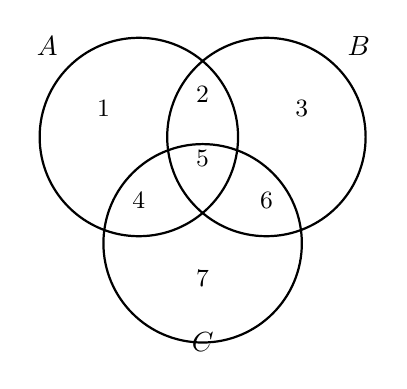
\begin{tikzpicture}[scale=0.9]
    % Three circles
    \draw[thick] (0,0) circle (1.4cm) node[above left=0.9cm] {$A$};
    \draw[thick] (1.8,0) circle (1.4cm) node[above right=0.9cm] {$B$};
    \draw[thick] (0.9,-1.5) circle (1.4cm) node[below=1cm] {$C$};
    % Region labels
    \node at (-0.5, 0.4) {\small 1};   % only A
    \node at (0.9, 0.6)  {\small 2};   % A∩B not C
    \node at (2.3, 0.4)  {\small 3};   % only B
    \node at (0.0,-0.9)  {\small 4};   % A∩C not B
    \node at (0.9,-0.3)  {\small 5};   % A∩B∩C
    \node at (1.8,-0.9)  {\small 6};   % B∩C not A
    \node at (0.9,-2.0)  {\small 7};   % only C
\end{tikzpicture}
\end{center}
\medskip

Using this labelling:
\begin{center}
\renewcommand{\arraystretch}{1.3}
\begin{tabular}{lll}
    \hline
    \textbf{Set expression} & \textbf{Regions shaded} & \textbf{Justification} \\
    \hline
    $A \cap B \cap C$
        & $\{5\}$
        & Elements in all three circles. \\[2pt]
    $(A \cap C) - B$
        & $\{4\}$
        & $A\cap C = \{4,5\}$; removing $B = \{2,3,5,6\}$ leaves $\{4\}$. \\[2pt]
    $(A \cap B) \cup (A \cap C)$
        & $\{2,4,5\}$
        & $A\cap B=\{2,5\}$, $A\cap C=\{4,5\}$; union $= \{2,4,5\}$. \\[2pt]
    $(A \cup B) \cap C$
        & $\{4,5,6\}$
        & $(A\cup B)\cap C=(A\cap C)\cup(B\cap C)=\{4,5\}\cup\{5,6\}$. \\[2pt]
    $(B \oplus C) \cap A$
        & $\{2,4\}$
        & $B\oplus C=\{2,3,4,7\}$; intersect with $A=\{1,2,4,5\}$ gives $\{2,4\}$. \\[2pt]
    $(A \cap C) \oplus B$
        & $\{2,3,4,6\}$
        & $A\cap C=\{4,5\}$; $(A\cap C)\oplus B=\{4\}\cup\{2,3,6\}=\{2,3,4,6\}$. \\[2pt]
    \hline
\end{tabular}
\end{center}

\begin{remark}
The identity $(A\cap B)\cup(A\cap C) = A\cap(B\cup C)$ (distribution) confirms
that regions $\{2,4,5\}$ are exactly those in $A$ that also lie in $B\cup C$.
\end{remark}

% ═════════════════════════════════════════════════════════════════════════════
\section{A Binary Relation on \texorpdfstring{$\R$}{R}}
% ═════════════════════════════════════════════════════════════════════════════

\begin{definition}
Define a relation $\Rel \subseteq \R \times \R$ by
\[
    x \;\Rel\; y \;\iff\; 1 \leq |x| + |y| \leq 2.
\]
\end{definition}

\subsection{Geometric description}

The condition $|x|+|y| \leq 2$ defines a square (rotated 45°) with vertices
at $(\pm 2, 0)$ and $(0, \pm 2)$, while $|x|+|y| \geq 1$ cuts out the
inner square with vertices at $(\pm 1, 0)$ and $(0, \pm 1)$. The relation
$\Rel$ is therefore the \emph{annular} region between these two $\ell^1$-balls.

\begin{center}
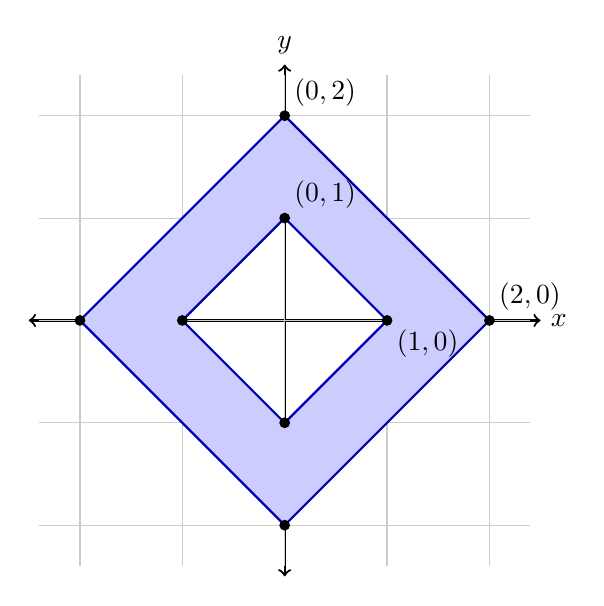
\begin{tikzpicture}[scale=1.3]
    \draw[<->, thick] (-2.5,0) -- (2.5,0) node[right] {$x$};
    \draw[<->, thick] (0,-2.5) -- (0,2.5) node[above] {$y$};
    \draw[gray!40, thin, step=1] (-2.4,-2.4) grid (2.4,2.4);

    % Shaded region between the two diamonds
    \begin{scope}[even odd rule]
        \fill[blue!20]
            (2,0) -- (0,2) -- (-2,0) -- (0,-2) -- cycle
            (1,0) -- (0,1) -- (-1,0) -- (0,-1) -- cycle;
    \end{scope}

    % Outer diamond boundary
    \draw[thick, blue!70!black]
        (2,0) -- (0,2) -- (-2,0) -- (0,-2) -- cycle;
    % Inner diamond boundary
    \draw[thick, blue!70!black]
        (1,0) -- (0,1) -- (-1,0) -- (0,-1) -- cycle;

    % Corner labels
    \foreach \pt in {(1,0),(0,1),(-1,0),(0,-1),(2,0),(0,2),(-2,0),(0,-2)}{
        \fill[black] \pt circle (1.5pt);
    }
    \node[below right] at (1,0)  {$(1,0)$};
    \node[above right] at (0,1)  {$(0,1)$};
    \node[above right] at (2,0)  {$(2,0)$};
    \node[above right] at (0,2)  {$(0,2)$};
\end{tikzpicture}
\end{center}

\subsection{Properties of \texorpdfstring{$\Rel$}{R}}

\begin{proposition}
$\Rel$ is not reflexive.
\end{proposition}
\begin{proof}
Take $x = 10$. Then $|x| + |x| = 20 > 2$, so $1 \leq |x|+|x| \leq 2$ fails.
Hence $x \cancel{\Rel} x$, and $\Rel$ is not reflexive.
\end{proof}

\begin{proposition}
$\Rel$ is symmetric.
\end{proposition}
\begin{proof}
Suppose $x \Rel y$, i.e.\ $1 \leq |x| + |y| \leq 2$. Then
\[
    |y| + |x| = |x| + |y|,
\]
so $1 \leq |y| + |x| \leq 2$, giving $y \Rel x$.
\end{proof}

\begin{proposition}
$\Rel$ is not antisymmetric.
\end{proposition}
\begin{proof}
Take $x = 0$ and $y = 1$. Then $|x|+|y| = 1$, so $x \Rel y$.
By symmetry, $y \Rel x$. But $x \neq y$, so antisymmetry fails.
\end{proof}

\begin{proposition}
$\Rel$ is not transitive.
\end{proposition}
\begin{proof}
Take $x = 0$, $y = 2$, $z = 0$. Then
\[
    |x|+|y| = 2 \in [1,2],\quad \text{so } x \Rel y,
\]
\[
    |y|+|z| = 2 \in [1,2],\quad \text{so } y \Rel z.
\]
But $|x|+|z| = 0 < 1$, so $x \cancel{\Rel} z$, and transitivity fails.
\end{proof}

% ═════════════════════════════════════════════════════════════════════════════
\section{A Partial Order via Divisibility}
% ═════════════════════════════════════════════════════════════════════════════

\begin{definition}
Let $P = \{n \in \N : n \mid 54\} = \{1,2,3,6,9,18,27,54\}$, and define a
relation $\preceq$ on $P$ by
\[
    a \preceq b \;\iff\; a \mid b.
\]
Then $(P, \preceq)$ is a \defn{partially ordered set} (poset).
\end{definition}

\subsection{Hasse diagram}

In the Hasse diagram, an upward edge from $a$ to $b$ indicates that $a \mid b$
and there is no element $c \in P$ with $a \mid c$ and $c \mid b$ strictly
(i.e.\ $b$ \emph{covers} $a$).

\begin{center}
\begin{tikzpicture}[scale=1.8,
    every node/.style={circle, draw, minimum size=7mm, font=\small}]
    % Nodes
    \node (1)  at (0,0)   {$1$};
    \node (2)  at (-1,1)  {$2$};
    \node (3)  at (1,1)   {$3$};
    \node (6)  at (0,2)   {$6$};
    \node (9)  at (2,2)   {$9$};
    \node (18) at (1,3)   {$18$};
    \node (27) at (3,3)   {$27$};
    \node (54) at (2,4)   {$54$};
    % Edges (covering relations only)
    \draw (1) -- (2);
    \draw (1) -- (3);
    \draw (2) -- (6);
    \draw (3) -- (6);
    \draw (3) -- (9);
    \draw (6) -- (18);
    \draw (9) -- (18);
    \draw (9) -- (27);
    \draw (18) -- (54);
    \draw (27) -- (54);
\end{tikzpicture}
\end{center}

\subsection{Greatest lower bounds and least upper bounds}

For elements $a, b \in P$:
\begin{itemize}
    \item $\mathrm{glb}\{a,b\} = \gcd(a,b)$ (the greatest common divisor of
          $a$ and $b$, provided it lies in $P$).
    \item $\mathrm{lub}\{a,b\} = \mathrm{lcm}(a,b)$ (the least common multiple,
          provided it lies in $P$).
\end{itemize}

Since $54 = 2 \cdot 3^3$, every divisor of $54$ is of the form $2^i 3^j$ with
$i \in \{0,1\}$ and $j \in \{0,1,2,3\}$, so $\gcd$ and $\mathrm{lcm}$ of any
two elements of $P$ remain in $P$.

\medskip
\noindent\textbf{Greatest lower bounds} ($\gcd$):
\[
\begin{array}{c|cccccccc}
    \mathrm{glb} & 1 & 2 & 3 & 6 & 9 & 18 & 27 & 54 \\
    \hline
    1  & 1 & 1 & 1 & 1 & 1 & 1  & 1  & 1  \\
    2  & 1 & 2 & 1 & 2 & 1 & 2  & 1  & 2  \\
    3  & 1 & 1 & 3 & 3 & 3 & 3  & 3  & 3  \\
    6  & 1 & 2 & 3 & 6 & 3 & 6  & 3  & 6  \\
    9  & 1 & 1 & 3 & 3 & 9 & 9  & 9  & 9  \\
    18 & 1 & 2 & 3 & 6 & 9 & 18 & 9  & 18 \\
    27 & 1 & 1 & 3 & 3 & 9 & 9  & 27 & 27 \\
    54 & 1 & 2 & 3 & 6 & 9 & 18 & 27 & 54 \\
\end{array}
\]

\noindent\textbf{Least upper bounds} ($\mathrm{lcm}$):
\[
\begin{array}{c|cccccccc}
    \mathrm{lub} & 1 & 2 & 3 & 6 & 9 & 18 & 27 & 54 \\
    \hline
    1  & 1  & 2  & 3  & 6  & 9  & 18 & 27 & 54 \\
    2  & 2  & 2  & 6  & 6  & 18 & 18 & 54 & 54 \\
    3  & 3  & 6  & 3  & 6  & 9  & 18 & 27 & 54 \\
    6  & 6  & 6  & 6  & 6  & 18 & 18 & 54 & 54 \\
    9  & 9  & 18 & 9  & 18 & 9  & 18 & 27 & 54 \\
    18 & 18 & 18 & 18 & 18 & 18 & 18 & 54 & 54 \\
    27 & 27 & 54 & 27 & 54 & 27 & 54 & 27 & 54 \\
    54 & 54 & 54 & 54 & 54 & 54 & 54 & 54 & 54 \\
\end{array}
\]

\subsection{Lattice structure}

\begin{proposition}
$(P, \preceq)$ is a lattice.
\end{proposition}

\begin{proof}
A poset is a lattice if and only if every pair of elements has a unique greatest
lower bound and a unique least upper bound. The tables above show that both
$\mathrm{glb}\{a,b\}$ and $\mathrm{lub}\{a,b\}$ exist and are unique for every
pair $\{a,b\} \subseteq P$. Hence $(P, \preceq)$ is a lattice.
\end{proof}

